%Document-Author: Bonato Paolo + Biggeri Mattia
%Document-Date: 2016/03/24
%Document-Description: Documento di Specifica tecnica del gruppo SWEeneyThreads 

\documentclass[a4paper]{article}
\usepackage[english, italian]{babel}
\usepackage[T1]{fontenc}
\usepackage[utf8]{inputenc}
\usepackage{url}
\usepackage{graphicx}
\usepackage[hidelinks]{hyperref}
\usepackage{booktabs}
\usepackage{eurosym}
\usepackage{tabularx}
\usepackage{pifont}
\usepackage[table]{xcolor}
\usepackage{float}
\usepackage[]{appendix}
\usepackage{ltxtable} 
\usepackage{geometry}
\geometry{margin=1in}
\usepackage{longtable}
\usepackage{multirow}

\graphicspath{{Immagini/}}

\newcolumntype{Y}{>{\centering\arraybackslash}X}
\newcolumntype{s}{>{\hsize=.21\hsize}X}
\newcolumntype{f}{>{\hsize=.37\hsize}X}
\newcolumntype{m}{>{\hsize=.42\hsize}X}
\newcolumntype{t}{>{\hsize=.1\hsize}X}
\newcolumntype{r}{>{\hsize=.3\hsize}X}
\newcolumntype{k}{>{\hsize=.4\hsize}X}

\renewcommand{\abstractname}{Tabella contenuti}

\begin{document}
	
	\begin{titlepage}
		% Defines a new command for the horizontal lines, change thickness here
		\newcommand{\HRule}{\rule{\linewidth}{0.5mm}} 
		\center  
		
		% HEADING SECTION
		\textsc{\LARGE SWEeneyThreads}\\[1.5cm] 
		\textsc{\Large Actorbase}\\[0.5cm] 
		\textsc{\large a NoSQL DB based on the Actor model}\\[0.5cm]
		
		
		% TITLE SECTION
		\HRule \\[0.4cm]
		{ \huge \bfseries Specifica Tecnica}\\[0.4cm] 
		\HRule \\[1.5cm]
		
		% AUTHOR SECTION
		\begin{minipage}{0.4\textwidth}
			\begin{flushleft} \large
				\emph{Redattori:}\\
				Bonato Paolo \\
				Biggeri Mattia
			\end{flushleft}
		\end{minipage}
		~
		\begin{minipage}{0.4\textwidth}
			\begin{flushright} \large
				\emph{Approvazione:} \\
				\emph{Verifica:} \\
				 
			\end{flushright}
		\end{minipage}
		
		%immagine
		\begin{figure}[H]
			\centering
			
\includegraphics[scale=0.8]{sweeney.png}
		\end{figure}
		\begin{center}
			Versione 1.0.2
		\end{center}
		% Date, change the \today to a set date if you want to be precise
		{\large \today}\\[3cm] 
		% Fill the rest of the page with whitespace
		\vfill  
	\end{titlepage}
	
	
	\tableofcontents
	
	\newpage 
	\section*{Diario delle modifiche}
		\begin{table}[H]
			\begin{tabularx}{\textwidth}{s f m X}
				\noalign{\hrule height 1.5pt}
				\rowcolor{orange!85} Versione & Data & Autore & Descrizione \\
				\noalign{\hrule height 0.5pt}
				1.0.2 & 2016-04-03 & \emph{Progettista} \newline Bonato Paolo & Accorpate le sezioni "Componenti", "Package" e "Classi" in "Componenti e classi". Riadattata la sezione "Metodo e formalismo di specifica" alla nuova struttura. Inserite le immagini 1 e 2. Apportate le correzioni indicate. \\
                \noalign{\hrule height 0.5pt}
				1.0.1 & 2016-03-26 & \emph{Progettisti} \newline Bonato Paolo \newline Biggeri Mattia \newline Padovan Tommaso \newline Tommasin Davide \newline Bortolazzo Matteo & Prima stesura di Architettura generale (sezinoe 3) e componenti (sezione 4)\\
				\noalign{\hrule height 0.5pt}
				1.0.0 & 2016-03-24 & \emph{Analisti} \newline Bonato Paolo \newline Biggeri Mattia & Creazione scheletro documento, stesura introduzione, definizione di metodo e formalismo di specifica. \\
				\noalign{\hrule height 1.5pt}
			\end{tabularx}
			\caption{Diario delle modifiche \label{tab:table_label}}
		\end{table}
	



	\newpage \section{Introduzione}
	\subsection{Scopo del documento}
		Il documento definisce la progettazione ad alto livello del progetto Actorbase.
		Verrà presentata l'architettura generale, le componenti, le classi e i design pattern utilizzati per realizzare il prodotto.
	\subsection{Scopo del prodotto}
		Il progetto consiste nella realizzazione di un DataBase NoSQL key-value basato sul modello ad 
		Attori con l'obiettivo di fornire una tecnologia adatta allo sviluppo di moderne 
		applicazioni che richiedono brevissimi tempi di risposta e che elaborano enormi quantità 
		di dati. Lo sviluppo porterà al rilascio del software sotto licenza MIT.
	\subsection{Glossario}
		Al fine di evitare ambiguità di linguaggio e di massimizzare la comprensione dei documenti, il 
      gruppo ha steso un documento interno che è il \emph{Glossario v1.3.0}. In esso saranno definiti, in modo
      chiaro e conciso i termini che possono causare ambiguità o incomprensione del testo.
	\subsection{Riferimenti}
		\begin{itemize}
			\item \textbf{Slide dell'insegnamento Ingegneria del software mod.A:} \\
			\url{http://www.math.unipd.it/~tullio/IS-1/2015/Dispense/E02.pdf}
			\item \textbf{Scala:} \\
			\url{http://www.scala-lang.org/}
			\item \textbf{Java:} \\
			\url{http://www.java.com/}
			\item \textbf{Akka:} \\
			\url{http://akka.io/}
		\end{itemize}
	\subsubsection{Normativi}
		\begin{itemize}
			\item \textbf{Norme di progetto:} \emph{Norme di progetto v1.3.3}
			\item \textbf{Capitolato d'appalto Actorbase (C1):} \\ 
			\url{http://www.math.unipd.it/~tullio/IS-1/2015/Progetto/C1p.pdf}
		\end{itemize}
		
		
	\newpage 
	\section{Tecnologie utilizzate}
	\subsection{Scala}
		Le possibili scelte dettate dal capitolato sono Java e Scala. Si è scelto di utilizzare Scala perché offre i seguenti vantaggi:
		\begin{itemize}
			\item \textbf{Concorrenza e distribuzione:} Ottimo supporto alla programmazione multi-threaded e distribuita, essenziale per la realizzazione di un prodotto responsive e scalabile.
			\item \textbf{Supporto di Akka:} Il linguaggio supporta la libreria Akka che è richiesta dal capitolato.
		\end{itemize}
		Inoltre il Committente ha espresso esplicitamente la sua preferenza sull'utilizzo di Scala.
		
	\subsection{Akka}
		L'utilizzo della libreria Akka è reso obbligatorio dal capitolato ed è la base del modello ad attori che costituisce il progetto.
	
	\newpage 
	\section{Descrizione dell'architettura}
		\subsection{Metodo e formalismo di specifica}
			Nell'esposizione dell'architettura del prodotto si procederà con un approccio di tipo top-down, ovvero dal generale al particolare.
			Inizialmente si descriveranno le tre componenti fondamentali: Client, Server e Driver; poi le componenti più piccole al loro interno, specificando i package e le classi che li compongono.
			Per ogni package saranno descritti brevemente il tipo, l'obiettivo e la funzione e saranno specificati eventuali figli, classi ed interazioni con altri package.
			Ogni classe sarà dotata di una breve descrizione e ne saranno specificate le responsabilità, le classi ereditate, le sottoclassi e le relazioni con altre classi.
			Successivamente saranno mostrati e descritti i diagrammi delle attività che coinvolgono l'utente.
			Infine si illustreranno degli esempi di utilizzo dei design pattern nell'architettura del sistema.
		\subsection{Architettura generale}
        	Il sistema ha un'architettura generale di tipo client-server.
            Il server ha un'architettura di tipo event-driven basata sul modello ad attori ed espone delle API tramite socket TCP.
            L'architettura del Client segue il design pattern Model-View-Controller con interfaccia da linea di comando e comunica con il server  grazie ad un driver tramite connessione TCP.
            
        \begin{figure} [H]
			\centering
			\includegraphics[scale=0.35]{Packages_Generale.png}
			\caption{Architettura generale, vista Package}
		\end{figure}
		
		\begin{figure} [H]
			\centering
			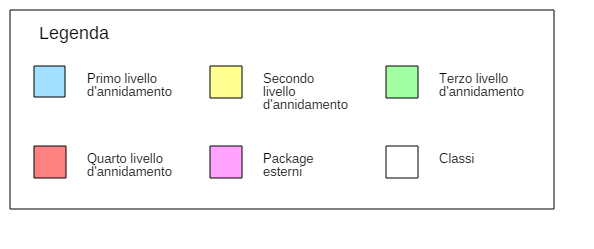
\includegraphics[scale=0.3]{Legenda.png}
			\caption{Legenda}
		\end{figure}
            \subsubsection{Server}
        	Le componenti principali del server sono gli attori:
            \begin{itemize}
				\item \textbf{Storekeeper:} Mantengono fisicamente in memoria le mappe chiave/valore.
                \item \textbf{Ninja:} Sono associati ad uno Storekeeper. Permettono di mantenere la consistenza del database anche nell'eventualità di un guasto. Se si perde uno Storekeeper, il Ninja a lui associato ne prende il posto. Per questa ragione, si trovano necessariamente in una macchina differente, ma rimangono costantemente in aggiornamento.
                \item \textbf{Storefinder:} Si occupano di ricevere richieste dall'esterno e instradarle ai rispettivi Storefinder, virtualmente ogni Storefinder definisce un indice sulla chiave della mappa. Il loro numero è veriabile e può essere configurato. Uno degli Storefinder è definito \textbf{main} e funge da punto di accesso al database.
                \item \textbf{Warehousemen:} Si interfaciano con gli Storekeeper e trascrivono persistentemente le rispettive mappe su disco.
                \item \textbf{Manager:} Ricevono le richieste di gestione degli attori di tipo Storekeeper, ad esempio sono responsabili del numero massimo di coppie chiave/valore contenute in un'istanza di Storekeeper.
			\end{itemize}
            
        \subsubsection{Client}
        	L'architettura del Client seguirà il design pattern MVC:
            \begin{itemize}
				\item \textbf{Model:}
                	Il Model è la componente che si occupa di comunicare con il server usando i metodi del driver e di notificare la View quando avviene un cambiamento nel suo stato.
                \item \textbf{View:}
                	La View è la componente che interagisce con l'utente mediante interfaccia a linea di comando. L'utente può usare il DSL per interrogare il Model. La View esegue delle \emph{state query} sul model per avere le informazioni aggiornate.
                \item \textbf{Controller:}
                	Il Controller è la componente che esegue il parsing dei comandi del DSL inseriti nella View e li notifica al Model.			
			\end{itemize}
        
        \subsubsection{Driver}
        	Il Driver è una libreria, invocando i metodi della quale è possibile effettuare richieste TCP verso le API esposte dal Server.
            
	\newpage 
	\section{Componenti e classi}
		\subsection{componente 1}
			% Immagine
			\subsubsection{Package}
				% Descrizione
				% Figli
				% Classi
				% Interazioni con altri package
			\subsubsection{Classi}
				% Descrizione
				% Responsabilità
				% Classi ereditate
				% Sottoclassi
				% Relazioni con altre classi
			
	\newpage 
	\section{Diagrammi delle attività}
	
	\newpage 
	\section{Design pattern}
	
	\newpage 
	\section{Stime di fattibilità e di bisogno di risorse}
	
	\newpage 
	\section{Tracciamento}
		\subsection{Tracciamento componenti-requisiti}
		\subsection{Tracciamento requisiti-componenti}
		
	\newpage 
	\section{Appendice}
	
	\cleardoublepage
	\addcontentsline{toc}{section}{\listfigurename}
	\listoffigures
	
	\cleardoublepage
	\addcontentsline{toc}{section}{\listtablename}
	\listoftables
		
\end{document}